\chapter{Objetivos y Metodología} 
\label{Chapter2} 
%----------------------------------------------------------------------------------------
%	SECTION 1
%----------------------------------------------------------------------------------------
Una vez  hemos enfocado el contexto en el que se va a desarrollar este trabajo,pasamos a describir los objetivos mas concretos que se pretenden cubrir en este TFG
\section{Objetivos}
Como objetivo global nos proponemos realizar varias practicas para la asignatura LTAW en el que se trabaja con tecnologias Web. En cada una de ella pretendemos emplear tecnologias que estan tomando mayor importancia al igual que proveer a los alumnos modelo de como deberia resolverse cada una de las practicas.
%-----------------------------------
%	SUBSECTION 1
%-----------------------------------
\subsection{Requisitos}
Se deben satisfacer los siguintes requisitos:
\begin{itemize}
\item Implementacion de nuevas tecnologias.
\item Proveer a los alumnos del aspecto que tiene que tomar las practicas.
\item Aportar nuevas funcionalidades en las practicas.
\end{itemize}
%----------------------------------------------------------------------------------------
%	SECTION 2
%----------------------------------------------------------------------------------------
\section{Metodologia y plan de trabajo}
La realizacion de todo proyecto necesita una metodologia a seguir con el que se planifica las tareas necesarias para llegar a nuesto objetivo. Por ello se ha seleccionado el modelo de desarrollo en espiral ya que es un modelo que se aplica habitualmente en la ingenieria de software.
\begin{figure}[!h]
\begin{center}
  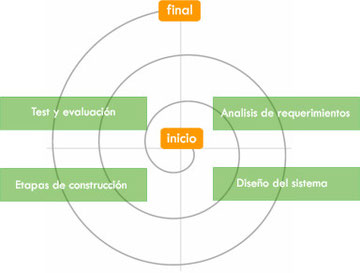
\includegraphics[width=0.6\linewidth]{Figures/modelo}
	\decoRule
	\caption[An Electron]{An electron (artist's impression).}
\label{fig:canvas}
\end{center}
\end{figure}
\\Este modelo define una serie de ciclos que se repiten continuamente hasta finalizar el proyecto, dividiendolo en subtareas mas sencillas en las que se establece un punto de control al final de cada una con el objetivo de evaluar el resultado y establece las nuevas tareas.
\\Durante  el tiempo que ha durado el proyecto se acordaron reuniones semanales aproximadamente con el tutor. En cada reunion se establecia los objetivos semanas y se evaluba los avances de acuerdo a la hoja de seguimiento. 
\\Para seguir el progreso del proyecto  disponiamos de una mediawiki \footnote{htto;/djadeor} de JdeRobot la que se actualizaba con los avances mas relevantes del proyecto. Aparte de disponer de esta plataforma trabajamos con el repositorio de GitHub \footnote{github-Wakter}  en el que se encuentra alojado el codigo fuente del proyecto.
\\Para finalizar este capitulo explicamos las distintas partes en las que se ha divido  el plan del proyecto.
\begin{enumerate}
\item \textbf{Aprendizaje de tecnologias web necesarias:} Estudiar y conocer distintas tecnologias  web en el  lado del servidor,cliente,BBDD y otras tecnologias que sirven de interconexion entre el cliente y el servidor.
\item \textbf{Seleccion de practicas}: Con los conocimientos adquiridos realizamos una propuesta que se ajuste a los conocimientos.
\item \textbf{Desarrollo de practicas}
\item \textbf{Experimentos:}En dos de las cuatro practicas se realizan experimentos en distintas situaciones para reflejar el comportamiento del desarrollo ente ellos.
\end{enumerate}
